% Created 2020-07-28 mar 10:02
% Intended LaTeX compiler: pdflatex
\documentclass[presentation,aspectratio=1610]{beamer}
\usepackage[utf8]{inputenc}
\usepackage[T1]{fontenc}
\usepackage{graphicx}
\usepackage{grffile}
\usepackage{longtable}
\usepackage{wrapfig}
\usepackage{rotating}
\usepackage[normalem]{ulem}
\usepackage{amsmath}
\usepackage{textcomp}
\usepackage{amssymb}
\usepackage{capt-of}
\usepackage{hyperref}
\usepackage{khpreamble, euscript}
\DeclareMathOperator{\atantwo}{atan2}
\newcommand*{\ctrb}{\EuScript{C}}
\newcommand*{\obsv}{\EuScript{O}}
\usetheme{default}
\author{Kjartan Halvorsen}
\date{\today}
\title{Control computarizado - Retroalimentación con observador}
\hypersetup{
 pdfauthor={Kjartan Halvorsen},
 pdftitle={Control computarizado - Retroalimentación con observador},
 pdfkeywords={},
 pdfsubject={},
 pdfcreator={Emacs 26.3 (Org mode 9.3.6)}, 
 pdflang={English}}
\begin{document}

\maketitle

\section{Apollo moon lander}
\label{sec:org5671638}
\begin{frame}[label={sec:orge1a9d61}]{Ejemplo - El módulo lunar de Apollo}
\begin{center}
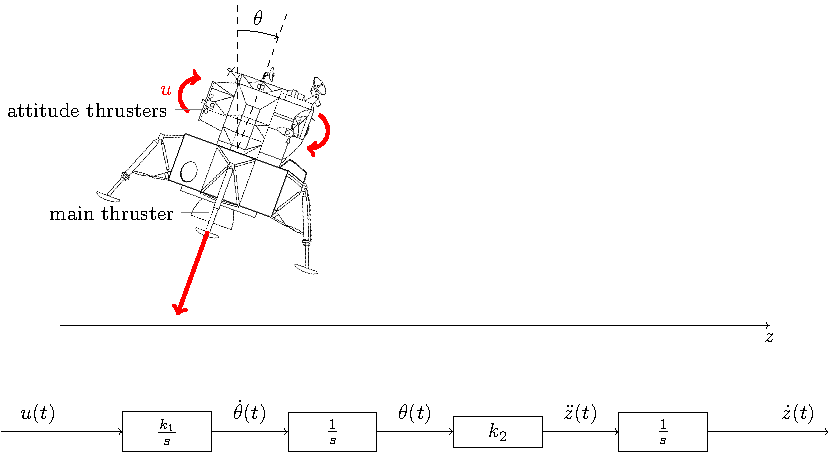
\includegraphics[width=\linewidth]{fig-apollo}
\end{center}
\end{frame}
\begin{frame}[label={sec:org8af05d3}]{Ejemplo - El módulo lunar de Apollo}
Variables del estado: \(x = \begin{bmatrix} x_1 & x_2 & x_3 \end{bmatrix}^T = \begin{bmatrix} \dot{\theta} & \theta & \dot{z} \end{bmatrix}^T\). Con dinamica
\[ \begin{cases} \dot{x}_1 =  \ddot{\theta} = k_1 u\\ \dot{x}_2 = \dot{\theta} = x_1\\ \dot{x}_3 = \ddot{z} = k_2\theta = k_2x_2 \end{cases} \]

\[ \dot{x} = \begin{bmatrix} \dot{x}_1\\\dot{x}_2\\\dot{x}_3\end{bmatrix} = \underbrace{\begin{bmatrix} \textcolor{red!60!black}{0} & \textcolor{red!60!black}{0} &\textcolor{red!60!black}{0} \\\textcolor{red!60!black}{1} & \textcolor{red!60!black}{0}& \textcolor{red!60!black}{0}\\ \textcolor{red!60!black}{0}& \textcolor{red!60!black}{k_2} &\textcolor{red!60!black}{0} \end{bmatrix}}_{A} \begin{bmatrix} x_1\\x_2\\x_3\end{bmatrix} + \underbrace{\begin{bmatrix} \textcolor{red!60!black}{k_1} \\ \textcolor{red!60!black}{0} \\\textcolor{red!60!black}{0}  \end{bmatrix}}_{B} u \]
\end{frame}

\begin{frame}[label={sec:orgdc23af2}]{Discretización - Módulo lunar de Apollo}
 \begin{align*}
  x(kh+h) &= \mathrm{e}^{Ah} x(kh) + \int_{0}^{h} \mathrm{e}^{As} B u(kh+h-s) ds\\
   &= \underbrace{\mathrm{e}^{Ah}}_{\Phi(h)} x(kh) + \underbrace{\left(\int_{0}^h \mathrm{e}^{As} B ds \right)}_{\Gamma(h)} u(kh)\\
   &= \begin{bmatrix} 1 & 0 & 0\\h & 1 & 0\\\frac{h^2k_2}{2} & hk_2 & 1\end{bmatrix} x(kh) + k_1 \begin{bmatrix} h\\ \frac{h^2}{2} \\ \frac{k_2 h^3}{6} \end{bmatrix} u(kh)
\end{align*}
\end{frame}


\section{State feedback with observer}
\label{sec:org8867cbe}
\begin{frame}[label={sec:orgd6bed3a}]{Control por retroalimentación de estados reconstruidos}
\end{frame}

\begin{frame}[label={sec:org74a0bb5}]{Control por retroalimentación de estados reconstruidos}
\begin{center}
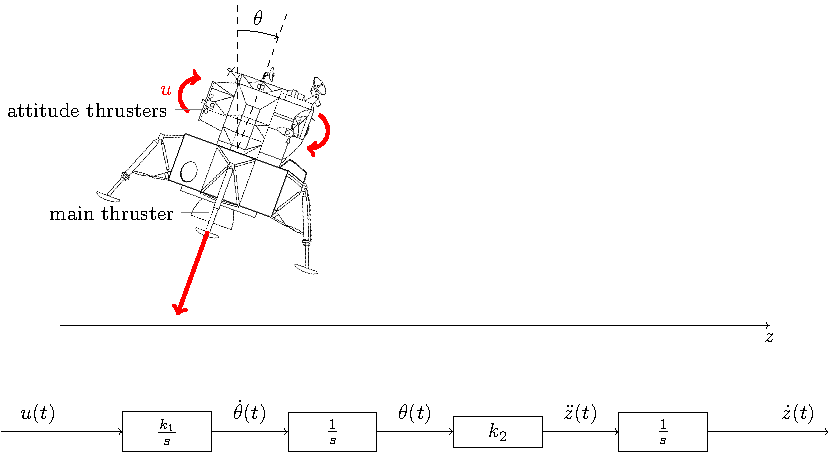
\includegraphics[width=0.9\linewidth]{fig-apollo}
\end{center}
\end{frame}

\begin{frame}[label={sec:orge5192cb}]{Retroalimentación de estados}
Dado
 \begin{equation}
 \begin{split}
  x(k+1) &= \Phi x(k) + \Gamma u(k)\\
  y(k) &= C x(k)
 \end{split}
 \label{eq:ssmodel}
\end{equation}
y medidas (o valores estimados) del vector de estado \(x(k)\). 

\alert{Retroalimentación lineal de estados} es la ley de control
\begin{equation*}
\begin{split}
 u(k) &= f\big((x(k), u_c(k)\big) = -l_1x_1(k) - l_2x_2(k) - \cdots - l_n x_n(k) + l_0u_c(k)\\
      &= -Lx(k) + l_0u_c(k), 
\end{split}
\end{equation*}
dónde \[ L = \bbm l_1 & l_2 & \cdots & l_n \ebm. \]
Sustituyende la ley de control en el modelo en espacio de estado \eqref{eq:ssmodel} da 
 \begin{equation}
 \begin{split}
  x(k+1) &= \left(\Phi -\Gamma L \right) x(k) + l_0\Gamma u_c(k)\\
  y(k) &= C x(k)
 \end{split}
 \label{eq:closedloop}
\end{equation}
\end{frame}



\begin{frame}[label={sec:org13f2b17}]{Diseño del observador}
Dado modelo
 \begin{equation*}
 \begin{split}
  x(k+1) &= \Phi x(k) + \Gamma u(k)\\
  y(k) &= C x(k)
 \end{split}
 \label{eq:ssmodel}
\end{equation*}
y medidas de la senal de salida \(y(k)\). 

El observador sería 
\begin{equation*}
\begin{split}
\hat{x}(k+1) &= \underbrace{\Phi \hat{x}(k) + \Gamma u(k)}_{\text{simulación}} + \underbrace{K\big(y(k) - C\hat{x}(k)\big)}_{\text{corrección}} = \left(\Phi - KC\right)\hat{x}(k) +  \Gamma u(k) + Ky(k)
\end{split}
\end{equation*}
con polos dados por los eigenvalores de la matriz \(\Phi_o = \Phi - KC\)

\alert{Regla de oro} Eliga los polos del observador (eigenvalores de \(\Phi-KC\)) por lo menos dos veces más rápidos que los polos (eigenvalores) de \(\Phi-\Gamma L\).
\end{frame}

\begin{frame}[label={sec:org879dcc9}]{Diseño del observador}
\alert{Regla de oro} Eliga los polos del observador (eigenvalores de \(\Phi-KC\)) por lo menos dos veces más rápidos que los polos (eigenvalores) de \(\Phi-\Gamma L\).

En tiempo continua (el plano s) hacer un polo dos veces más rápido significa mover el polo a una distancia doble del origen. Entonces, con el polo discreto \(p_1\) el polo discreto en 
\[ p_2 = \text{exp}\left( 2 \frac{\ln p_1}{h} h\right) = \text{exp} \big( 2 \ln p_1 \big)\]
corresponde a una respuesta dos veces más rapida.
\end{frame}

\begin{frame}[label={sec:orgc512225}]{Control por retroalimentación de estados reconstruidos}
Se puede separar el problema del diseño del controlador en dos
\begin{enumerate}
\item Diseñar el vector de ganancias \(\textcolor{orange!80!black}{L}\) en la ley de control
\[ u(k) = -\textcolor{orange!80!black}{L} \hat{x}(k) + l_0 u_c(k)\]
para obtener buen seguimiento a referencia.
\item Diseñar el vector de ganancias \(\textcolor{red}{K}\) en el observador 
\begin{equation*}
\begin{split}
\hat{x}(k+1) &= \Phi \hat{x}(k) + \Gamma u(k) + \textcolor{red}{K} \big(y(k) - C\hat{x}(k)\big)
\end{split}
\end{equation*}
para obtener una balancia entre rechazo a perturbaciones y sensibilidad a ruido de medida.
\end{enumerate}
\end{frame}

\begin{frame}[label={sec:orgbe44045}]{Matlab/simulink}
\end{frame}

\begin{frame}[label={sec:orgafeac82}]{Calculo de la ganancia del observador}
Una matriz \(M\) y su transponada \(M\transp\) tienen los mismos eigenvalores. Entonces,  el problema de determinar las ganancias \(K\) para obtener eigenvalores deseados de
\[\Phi- KC\] es equivalente de determinar las ganancias \(K\) en 
\[(\Phi-KC)\transp = \Phi\transp - C\transp K\transp.\]
Este último problema tiene la misma forma como el problem de determinar \(L\) para obtener eigenvalores deseados de 
\[\Phi - \Gamma L\]

Entonces, se puede usar el mismo método en matlab para calcular los dos vectores de ganancia, \(L\) y \(K\)
\end{frame}

\begin{frame}[label={sec:orgdd489e9},fragile]{Calculo de la ganancia del observador}
 \begin{enumerate}
\item \alert{Método de Ackerman} 
\begin{verbatim}
K = (acker(Phi', C', po))'
\end{verbatim}
\item \alert{Método numericamente estable} 
\begin{verbatim}
K = (place(Phi', C', pd))'
\end{verbatim}
\end{enumerate}
\end{frame}



\begin{frame}[label={sec:orgddbb34d}]{Matlab}
\end{frame}
\begin{frame}[label={sec:org784503f}]{Actividad}
En grupos: 
\begin{enumerate}
\item Agrega simulación de una perturbancia constante a la salida del sistema (pero antes de la medición). Esa perturbación representa un error de modelación. Simula un escalón positivo unitario occurriendo en \(t=10\)s
\item Determina la desviación máxima en la velocidad en respuesto a la perturbancia.
\item Determina las ganancias \(K = \bbm k_1 & k_2 & k_3 \ebm\transp\) para un observador \emph{dead-beat}. Es decir con todos los polos en el origen. Cómo cambia la desviación en la respuesta a la perturbancia?
\item Cambió la respuesta al escalón en la referencia al cambiar a un observador dead-beat?
\end{enumerate}
\end{frame}
\end{document}